%%%%%%%%%%%%%%%%%%%%%%%%%%%%%%%%%%%%%%%%%%%%%%%%%%%%%%%%%%%%%%%%%
% Contents: Things you need to know
% $Id$
%%%%%%%%%%%%%%%%%%%%%%%%%%%%%%%%%%%%%%%%%%%%%%%%%%%%%%%%%%%%%%%%%

\chapter{Things You Need to Know}
\begin{intro}
	Road tracking is one of the most challenging topics recently. It aims to automatically guide a car through the correct track without crashing other cars or objects. Deep reinforcement learning is considered as one of the most proficient methods that can be applied to address the road tracking issue. It combines reinforcement learning and deep learning. We model the process as a Markov Decision Process (MDP), where the deep reinforcement learning starts from a state, pick the best action by optimising considered rewards and produces a new state. The new state is then utilized as a current state, and the process continues.  

Different tracking tasks were considered in the literature as:
\begin{itemize}
	\item \underline{Tracking Object:} In 2000, Grigore and Grigore proposed a tracking system controller by using a recurrent neural network with the reinforcement learning \cite{Grigore2000Reinforcement}. In 2010, Cohen and Pavlovic suggested an effective and vigorous real-time tracker. The tracker utilized the reinforcement learning and it was applied to tracking personal faces \cite{Cohen2010Reinforcement}. In 2004, Liu and Su proposed an object tracking method by exploiting the reinforcement learning. The reinforcement learning was employed here to determine the features of the tracking object \cite{Liu2004Reinforcement}. In 2017, Supan\v{c}i\v{c} and Ramanan constructed a learning policy for tracking objects. The reinforcement learning was applied to video streams to provide on-line decision \cite{Supancic2017Tracking}. 
	\item \underline{Different Tracking Issues:} In 2009, Jinlin \textit{et al.} presented a velocity tracking control approach. The authors utilized the neuro-fuzzy technique with the Q-learning in their work \cite{Jinlin2009Neurofuzzy}. In 2011, Hall \textit{et al.} illustrated a single and double pendulum tracking model. A traditional control, Bayesian computations and reinforcement learning were employed in this publication \cite{Hall2011Reinforcement}. In 2013, Sootla \textit{et al.} described a tracking periodic gene repressilator. The fitted Q iteration algorithm was applied to one dimensional signals in this study \cite{Sootla2013On}. In 2015, Wei \textit{et al.} explained tracking a maximum power for wind speed conversion systems. In this paper, a model-free Q-learning method was exploited \cite{Wei2015Reinforcement}. 
	\item \underline{Deep Leaning Tracking:} In 2017, Perot \textit{et al.} investigated tracking roads of a driving car. A deep reinforcement learning was used \cite{Perot2017End}. The main problem in this work is that the driving car oscillates around the main road track. This is due to the selected reward in this study, where it utilized the oriented angle of the road with the car speed. In 2017 and 2018, Yun \textit{et al.} approached an action-decision network (ADNet) to track objects. The ADNet is a deep reinforcement learning network and it was applied in a quite complicated way, where a pre-trained Convolutional Neural Network (CNN) was firstly employed then the reinforcement learning was utilized \cite{Yun2017Action}\cite{Yun2018Action}. 
\end{itemize}

It can be seen from the literature that the majority of tracking studies were focused on tracking object problems as in \cite{Grigore2000Reinforcement}\cite{Cohen2010Reinforcement}\cite{Liu2004Reinforcement}\cite{Supancic2017Tracking}. Other work considered different tracking tasks such as: tracking and controlling velocity \cite{Jinlin2009Neurofuzzy}, tracking periodic gene repressilator \cite{Sootla2013On}, tracking single and double pendulum \cite{Hall2011Reinforcement}, tracking maximum powers for wind speed conversion systems \cite{Wei2015Reinforcement}. Only several studies were concentrated on utilizing the deep learning in order to address tracking issues such as \cite{Yun2017Action,Yun2018Action}. 

Our work contributes to this area by suggesting an effective road tracking procedure and employing the MDP based on the deep reinforcement learning, where states are used as inputs; rewards are utilized to evaluate the tracking policy and actions are predicted to provide new states. Efficient coding for various road tracking possibilities has been considered such as turning to the left or right and recognizing crossing object(s). This study can be exploited for driving car applications such as driverless (or automatic driving). 

After the introduction, this paper is organized as follows: Section 2 states the methodology with the theoretical concepts, Section 3 discusses the results and Section 4 concludes the paper.
\begin{figure*}[!t]
	\centering
	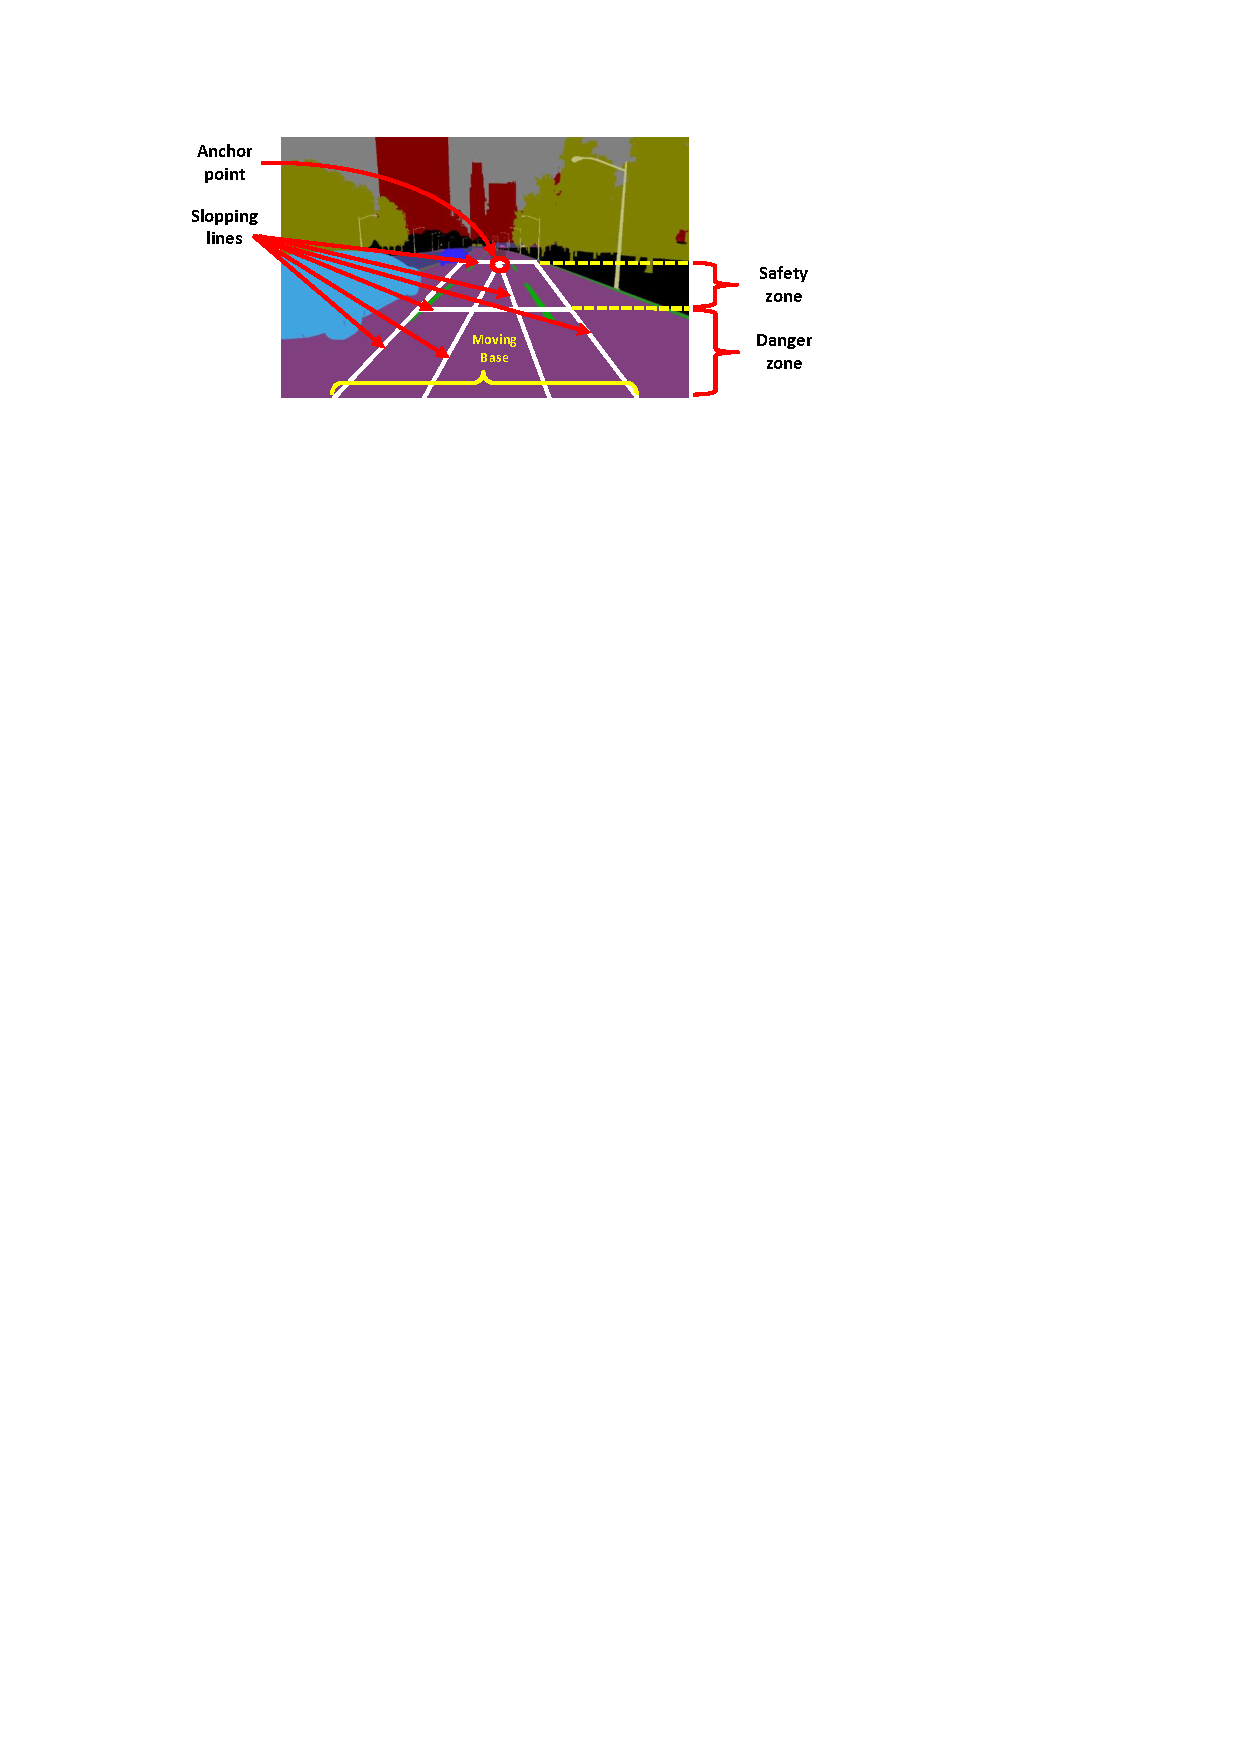
\includegraphics[scale=.9,trim=3cm 22.5cm 7.1cm 2cm,clip]{segmentation_regions2.pdf}
	\caption{The suggested front view road tracking zones, lines and anchor point}
	\label{Fig:segmentation_regions1}
\end{figure*}
\begin{figure*}[!t]
	\centering
	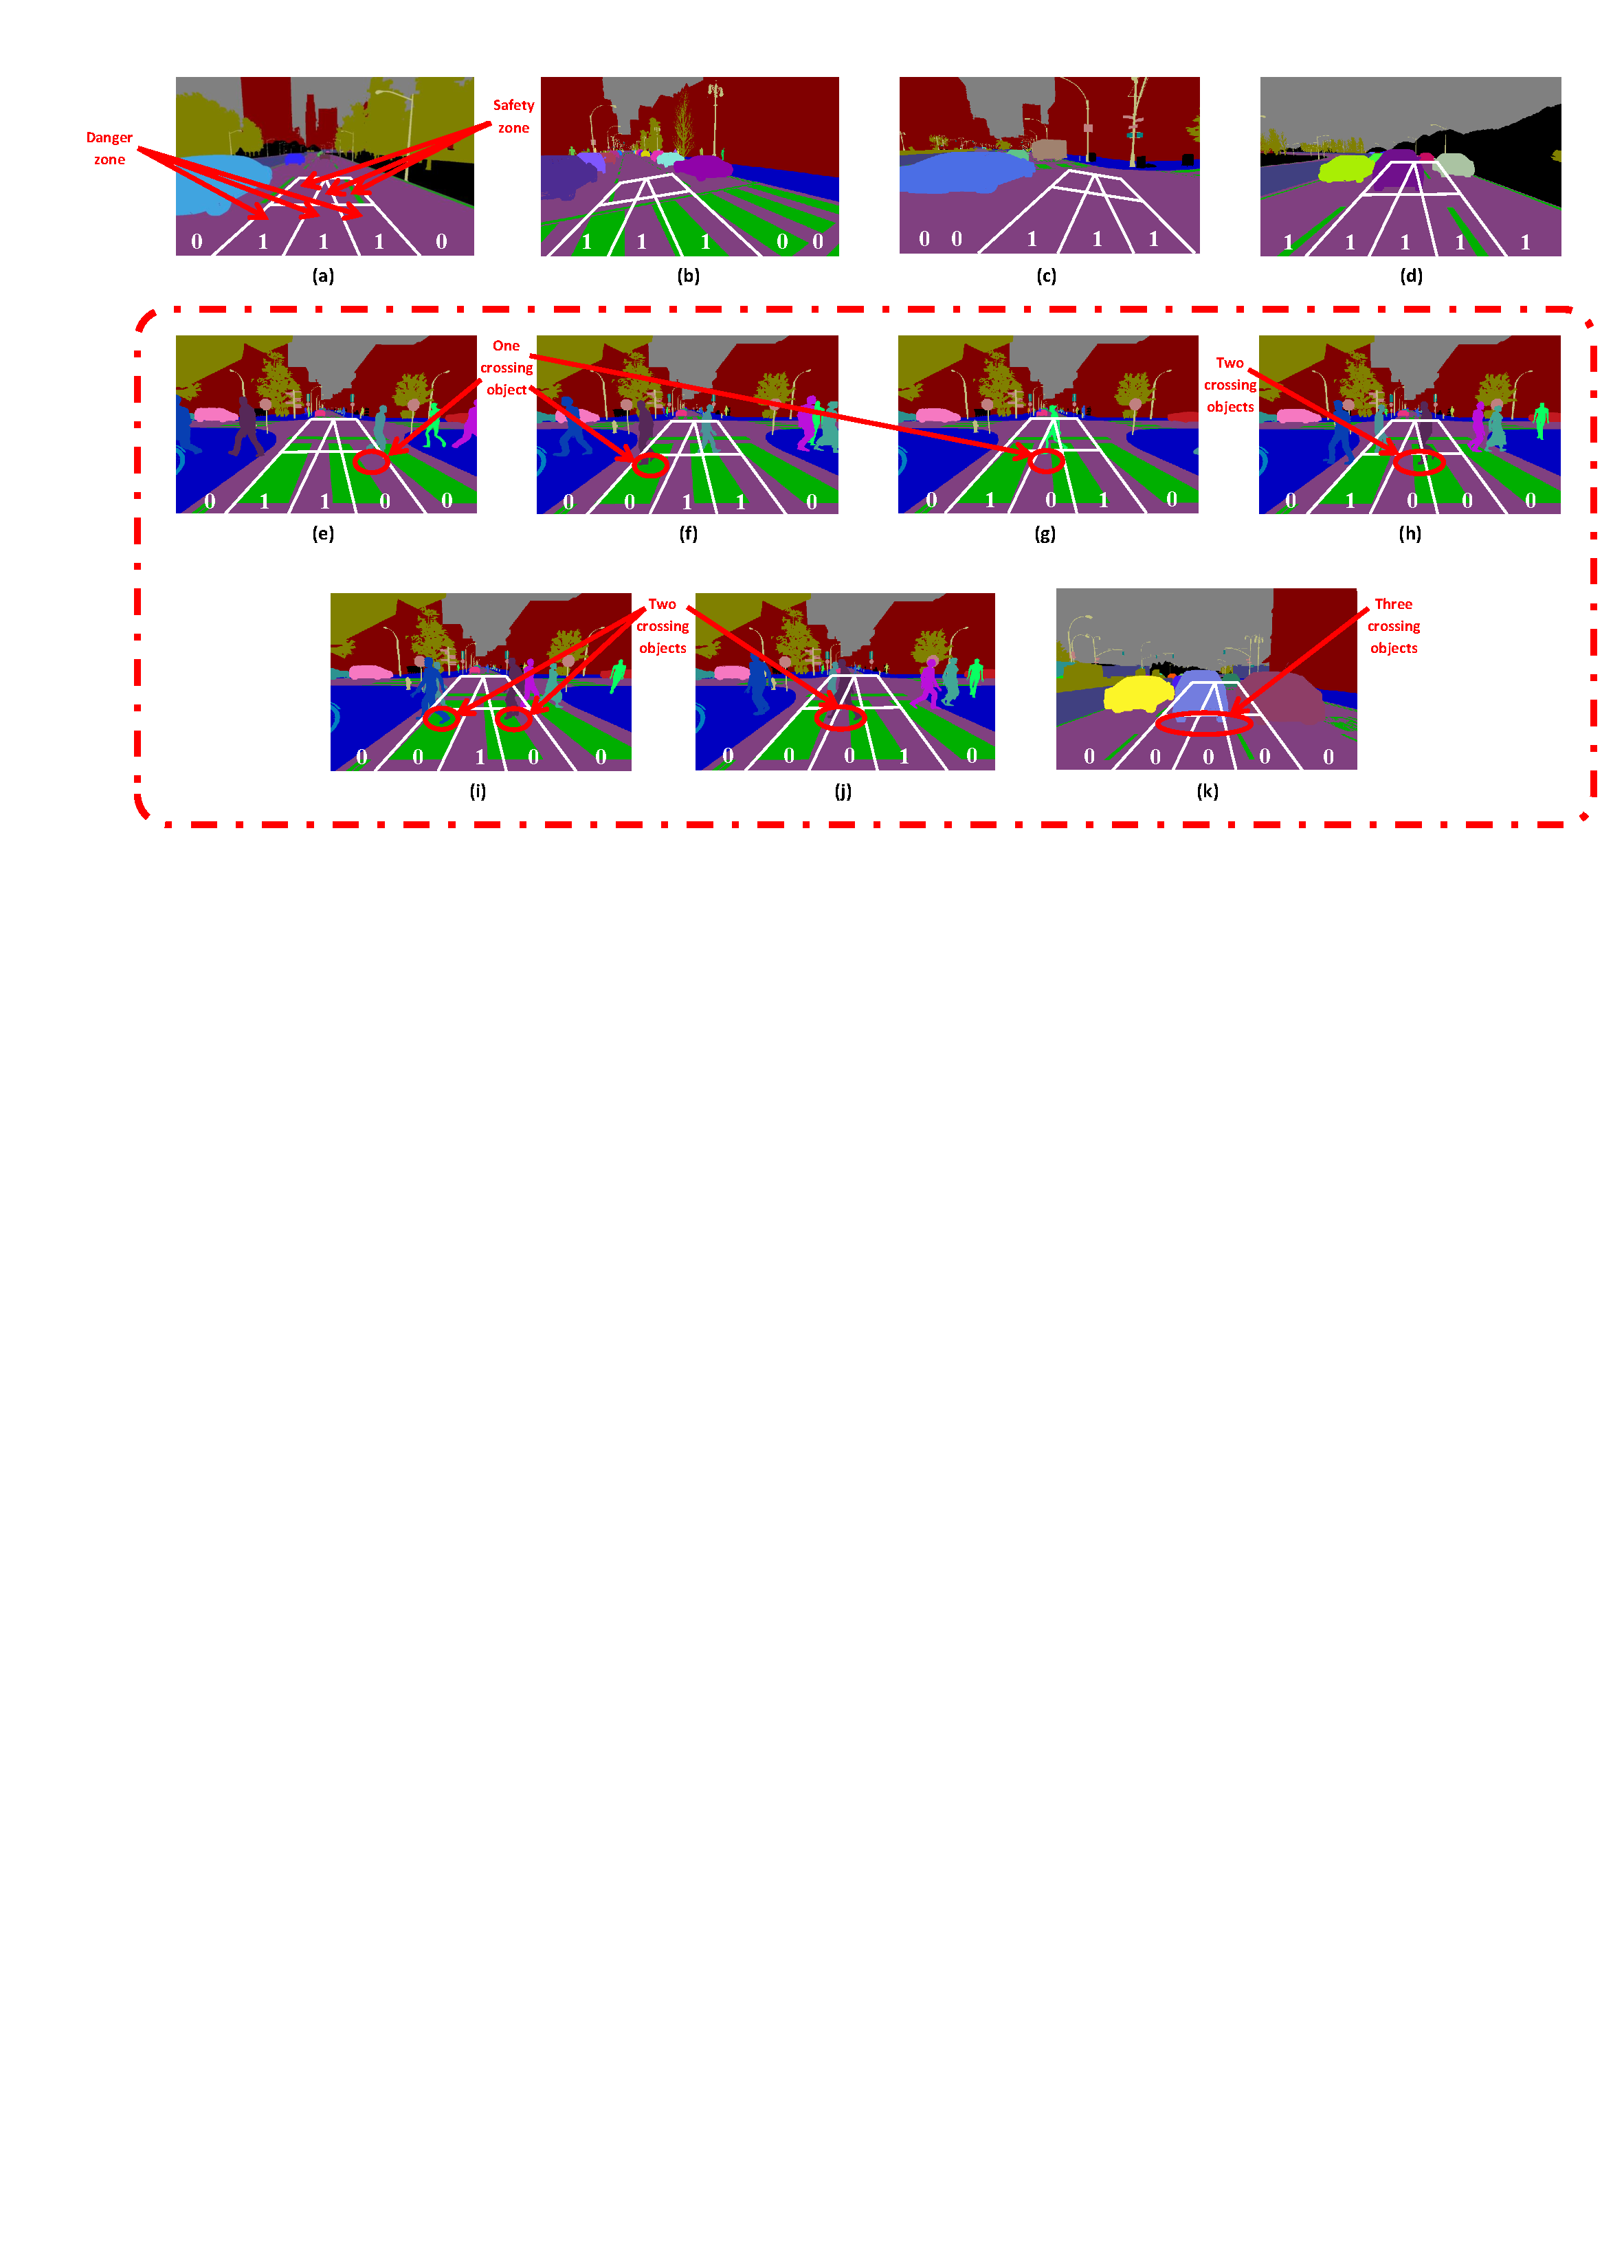
\includegraphics[scale=.4,trim=2cm 35cm 0cm 2cm,clip]{segmentation3.pdf}
	\caption{The road tracking motivations of segmented images: (a) the straight forward direction, (b) turning left direction, (c) turning right direction, (d) reverse or backward direction, (e-g) stopping action because of a single crossing object, (h-j) stopping action because of two crossing objects and (k) stopping action because of three crossing objects}
	\label{Fig:segmentation}
\end{figure*}
\begin{figure*}[!h]
	\centering
	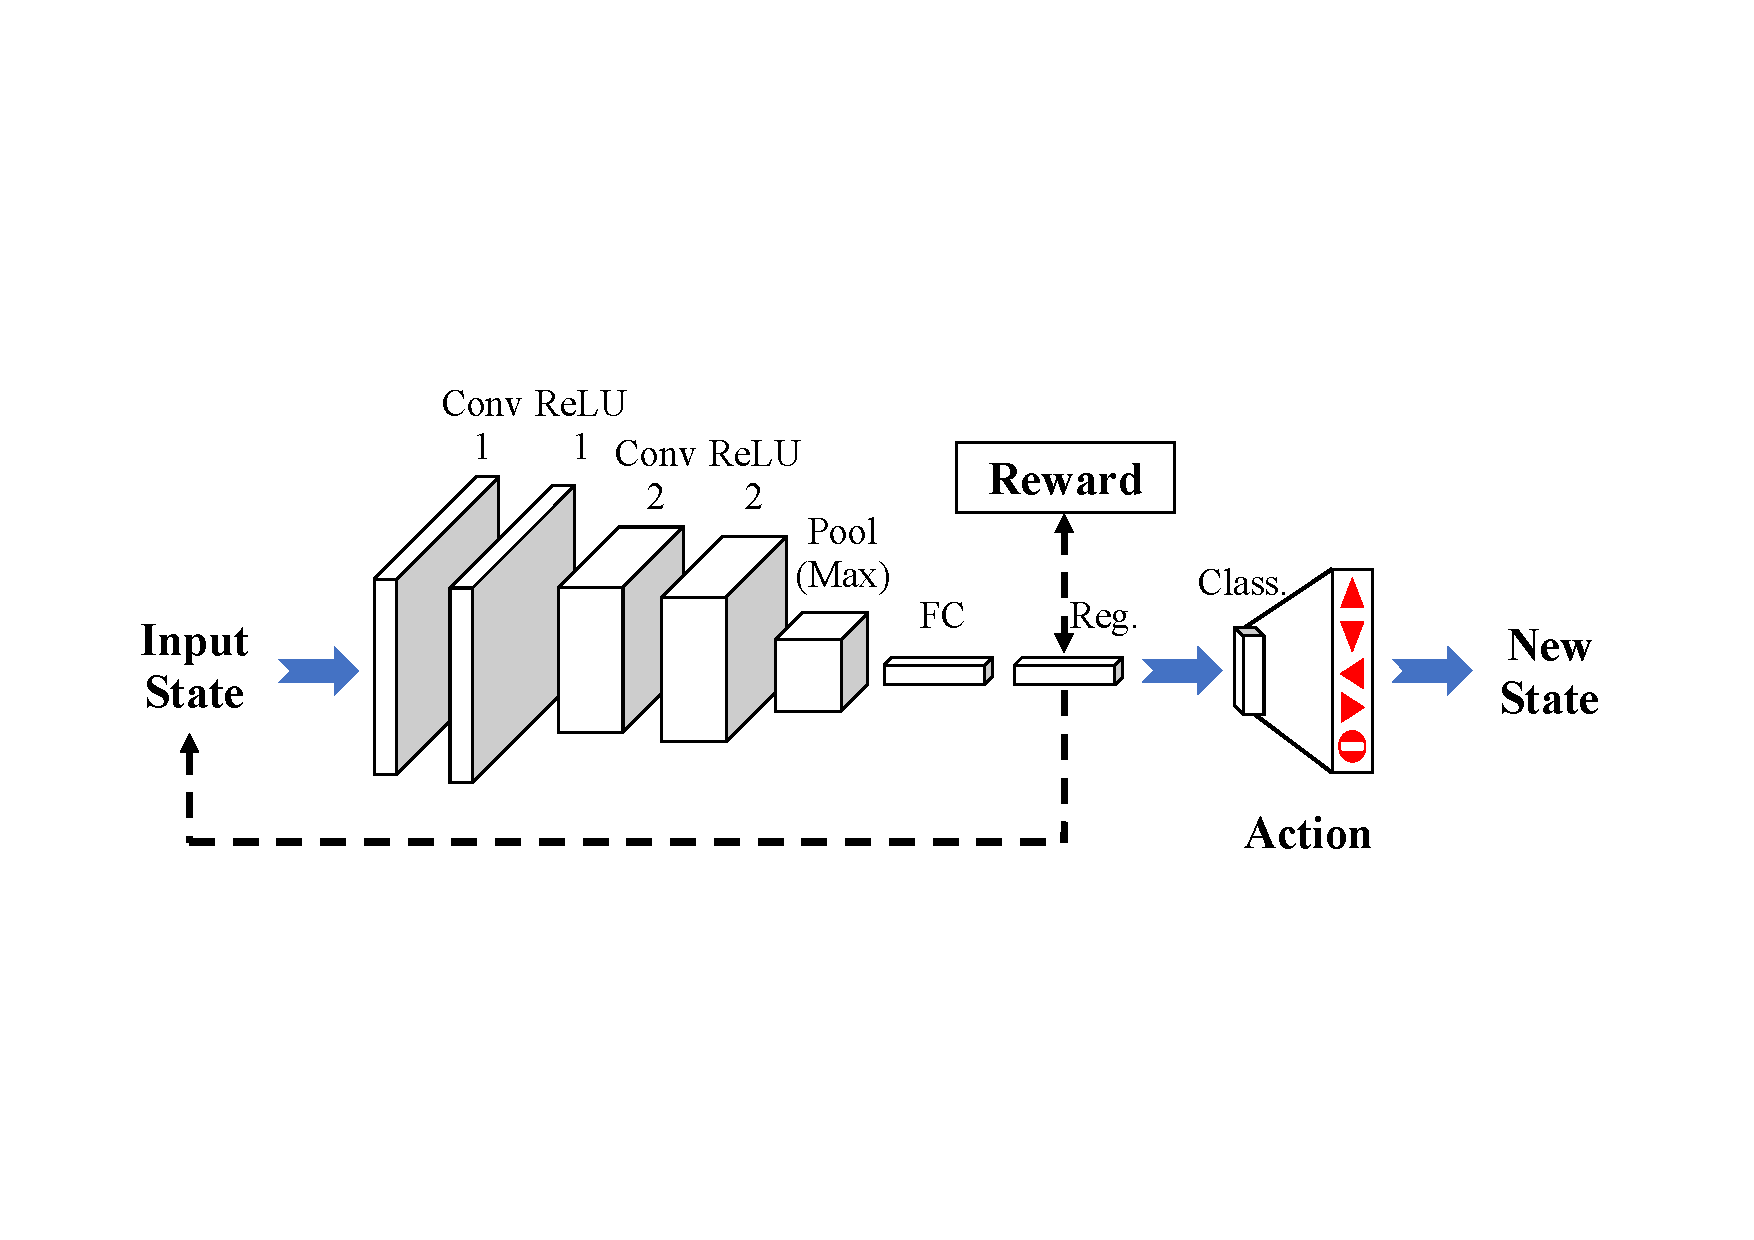
\includegraphics[scale=.65,trim=2cm 5.5cm 2cm 5.5cm,clip]{Deep_Reinf_Net1.pdf}
	\caption{The main design of the proposed DRL-RT. It consists of two conventional layers, two ReLU layers, a pooling layer, a fully connected layer, a regression layer and a classification layer}
	\label{Fig:Deep_Reinf_Net}
\end{figure*}
\end{intro}
